
% ====================================
% chapter 1
% ====================================

\chapter{序章}

% ページ番号をリセット
\setcounter{page}{1}
% ページ番号の付け方をromanからarabicに変えておく
\pagenumbering{arabic}


\section{背景}

\subsection{コーヒーの需要}
コーヒーは世界中で様々な形で飲まれており,近年日本でもコーヒーの需要は増加傾向にある.図\ref{fig_syouhi}は日本国内における年間のコーヒー消費量の推移である.1996年以降コーヒー消費量は増加を続け2016年には47万[t]を超える消費量を見せている.特に嗜好品としてのコーヒーがブームを迎えており,スペシャルティコーヒーと呼ばれる品質を重視したコーヒーの需要が高まっている

スペシャルティコーヒーとは「消費者(コーヒーを飲む人)の手に持つカップの中のコーヒーの液体の風味が素晴らしい美味しさであり,消費者が美味しいと評価して満足するコーヒーであること.」と定義づけられており,カップの中の風味が素晴らしい美味しさであるためには,コーヒーの豆(種子)からカップまでの総ての段階において一貫した体制・工程・品質管理が徹底していることが必須であるとされている.具体的には生産国における管理・処理が適切になされ,適切な輸送と保管により劣化のない状態で焙煎された高品質なコーヒー豆を用いて適切な抽出が行われたものである必要がある.

\begin{figure}[]
  \begin{center}
    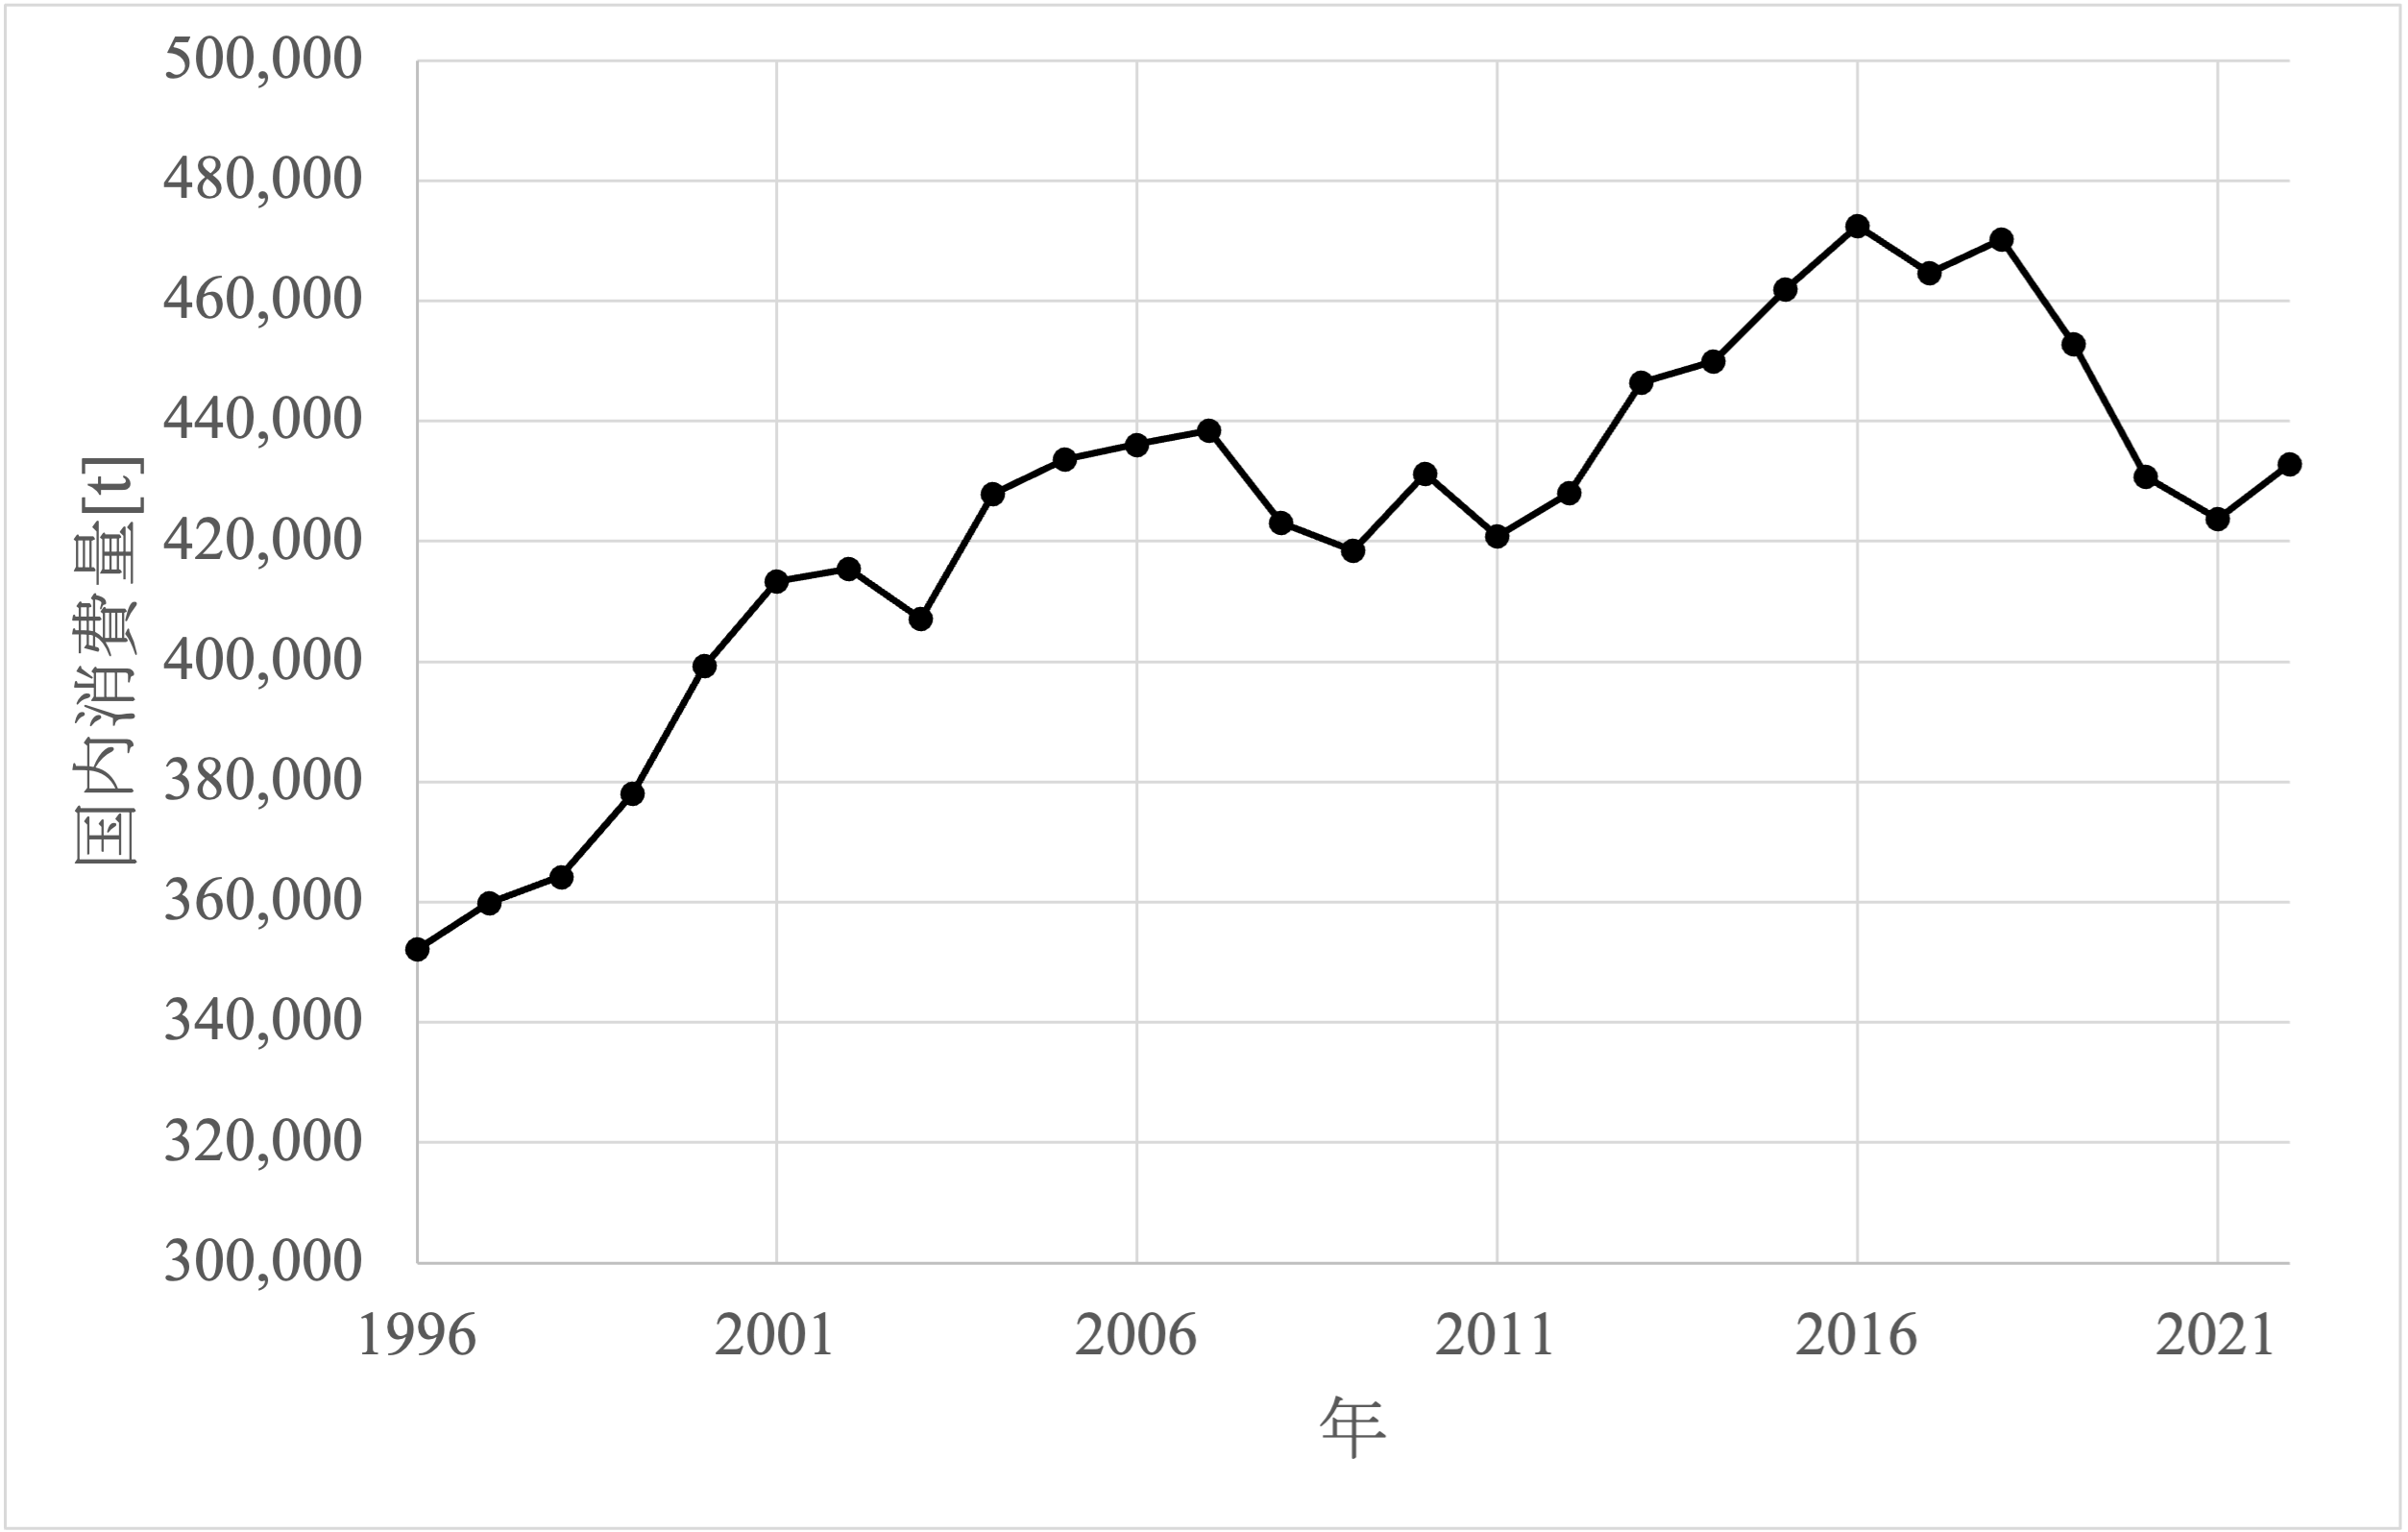
\includegraphics[scale = 0.5]{./chapter1/coffee_syouhi.png}
    \caption{Coffee consumption in Japan}
    \label{fig_syouhi}
  \end{center}
\end{figure}

\subsection{欠点豆とハンドピック}
近年のスペシャルティコーヒーのブームにより高品質なコーヒー豆が求められているが,コーヒー生豆において欠点豆と呼ばれるものが存在する.
欠点豆とはコーヒー生豆における,虫食いや欠けのあるような不良な豆のことである.以下に欠点豆の種類とその問題点についてまとめる.
\begin{itemize}
  \item カビ臭豆:不完全な乾燥や湿気を帯びた状態での輸送・保管が原因となり,青カビや白カビが発生した豆のこと.除去しなければコーヒー液自体にカビ臭が付着してしまう.
  \item 発酵豆:生産時や輸送中に発行が進み,菌が繁殖してしまっている豆のこと.異臭の原因になる.
  \item 貝殻豆:乾燥不良や異常勾配で発生する,センターカットから割れてしまった豆を指す.煎りムラの原因になり,焙煎時間が長くなると着火の危険性まで出てくる.
  \item 虫食い豆:コーヒーチェリーに産み付けられた蛾の幼虫がコーヒー豆の内部を食べることによってできた穴の空いたコーヒー豆のこと.濁りや異臭の原因になる.
  \item ピーベリー:発育不良によって通常コーヒーチェリー内部に2つあるコーヒー豆が1つの状態で育ってしまったもの.単体での味への影響はないが煎りムラの原因になる.
\end{itemize}
これらの欠点豆を選別しないまま焙煎を行なってしまうと煎りムラの原因や風味を劣化させる原因となってしまうため取り除く必要があるが,その際人間がコーヒー豆を目視で判別し手で取り除く「ハンドピック」と呼ばれるものを行なっている.
しかし,ハンドピックにはいくつかの問題が存在する.1つ目は生産地でハンドピックをすると,売り出すコーヒー豆の減少や作業量の増加からコーヒー豆の価格が高騰してしまうこと.2つ目は生産地でハンドピックをしたとしても輸送や保管の段階でコーヒー豆が劣化してしまい,輸入後のハンドピックが避けられないこと.3つ目はハンドピックそのものの労力が大きいことである.生産地から販売店までの商通で安価に精度良く選別することはできないため,販売店や個人でのハンドピックが必須であるが,それには大きな時間と労力が費やされている.

\section{目的}
ハンドピックにかかる大きな労力を低減するため,本研究では機械学習を用いてコーヒー生豆の良否判定を行う.先行研究ではConvolutional Neural Network(以下,CNN)を用いた判別を実現している.しかし,CNNの重みは浮動小数のため計算コストが高い.販売店や個人での利用を考えると,装置の小型化や省電力化が求められるため,将来的にFPGAやマイコンなどの計算リソースの少ないデバイスで制御したい.そこでBinaryConnectという手法を用いてNeural Network中の重みの2値化を目指す.通常,浮動小数で表されるCNNの重みは32bitや64bit分のメモリを消費するが,BinaryConnectを用いれば重みは1bitで表すことができる.これにより,メモリの消費を減らすことができるうえ,乗算機の数も減らすことができる.本稿ではCNNとBinalyConnectを用いてコーヒー生豆の良否判定精度を実験により比較し,BinaryConnectの有効性を検証する.
